\documentclass{beamer}
\usepackage{animate}
\usepackage{multimedia}
\usepackage[english,russian]{babel}

\usepackage{pgfpages}
\setbeameroption{show notes on second screen}
%https://tug.ctan.org/macros/latex/contrib/beamer/doc/beameruserguide.pdf

\usepackage[T2A]{fontenc}
\usepackage[utf8]{inputenc}

\setbeamertemplate{caption}[numbered]

\usetheme{CambridgeUS}
\usecolortheme{dolphin}


\title[Теория света и цвета]{Теория света и цвета. Методы представления графической информации}
\author[Быковских Д.А.]{Быковских Дмитрий Александрович}
\date{16.09.2023}

\if 0

https://gamedev.ru/code/terms/ToneMapping
https://gamedev.ru/code/terms/HDR
https://habr.com/ru/articles/709110/
https://en.wikipedia.org/wiki/Tone_mapping
https://en.wikipedia.org/wiki/High_dynamic_range
взять картинку
https://www.lesmer.ru/blog/hdr-and-tone-mapping
динамическое
http://webos-forums.ru/post153883.html
формула
https://wiki5.ru/wiki/Tone_mapping
https://www.researchgate.net/publication/338167112_Tone_mapping_for_video_data
https://ru.wikipedia.org/wiki/%D0%A6%D0%B2%D0%B5%D1%82#%D0%90%D1%85%D1%80%D0%BE%D0%BC%D0%B0%D1%82%D0%B8%D1%87%D0%B5%D1%81%D0%BA%D0%B8%D0%B5_%D1%86%D0%B2%D0%B5%D1%82%D0%B0
\fi

\begin{document}
\begin{frame}
	\titlepage
\end{frame}
%\section{Обзор}
\begin{frame}{Содержание}
		\begin{itemize}
			\item 
			Теория света
			\item
			Теория цвета
		\end{itemize}
	\end{frame}
	
	\begin{frame}{Теория света}

		\begin{figure}
					\includegraphics[width=\textwidth]{images/light\_range.jpeg}
					\caption{Видимый диапазон света}
		\end{figure}
				
				\note{
					% https://habr.com/ru/articles/473620/
					Свет — это электромагнитные (ЭМ) волны.
					
					Цвет характеризуется тремя величинами:
					
					Тон — это разные цвета (разные длины волн): синий, красный, зелёный.
					
					Насыщенность: розовый — это ненасыщенный красный.
					
					Светлота: розовый — это светло-красный, а бордовый — тёмно-красный.
				
					Зеленый цвет находится по середине, поэтому лучше всего воспронимает человеческое зрение.

					Дополнительные термины:

					Гамут --- охват цвета.

					Гамма --- охват яркости.
				}
			
	\end{frame}

	\begin{frame}{Спектральное распределение излучения}
		\begin{figure}
			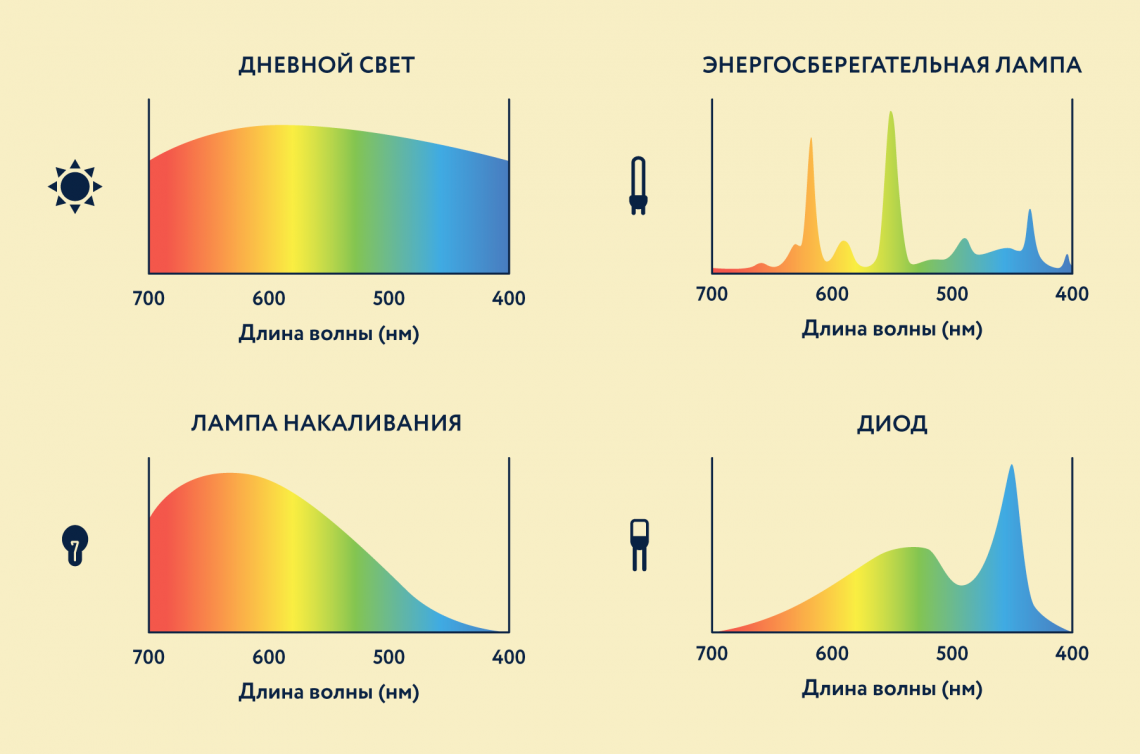
\includegraphics[width=0.6\textwidth]{images/спектральное-распределение-излучения-ИС.png}
			\caption{Спектральное распределение излучения различных источников света}
		\end{figure}
		\note{
			Оттенки серого (в диапазоне белый — чёрный) носят парадоксальное название ахроматических, т.е. бесцветных цветов. Парадокс разрешается, когда становится ясно, что под «отсутствием цвета» здесь понимается, естественно, не отсутствие цвета как такового, а отсутствие цветового тона, конкретного оттенка спектра. Наиболее ярким ахроматическим цветом является белый, наиболее тёмным — чёрный. 

		}
	\end{frame}

	\begin{frame}{Строение человеческого глаза}
		\begin{figure}
			\includegraphics[width=0.6\textwidth]{images/Schematiheskay\_diagrama\_the\_human.png}
			\caption{Оптическая система глаза}
		\end{figure}
		\note{
			{
				\scriptsize
			%Почему небо синее? Ответ: Рэлеевское рассеяние.

			Почему мы видим зелёные растения зелёными? 
			
			Потому что они поглощают весь видимый свет, кроме зелёной части, которая отражается и попадает на сетчатку.

			
			
			Баланс белого (ББ).
			Человеческое зрение колебрует поступающий свет.
			Такая автокоррекция цвета в зрительной системе потребовалась нам по многим причинам — одна из них, чтобы мы могли адекватно различать цвет объектов в разных условиях освещения.


			Палочки содержат пигмент родопсин. Его наибольшая чувствительность находится в области около 510 нм — бирюзовый цвет.

			Колбочки содержат пигмент йодопсин в трёх вариациях. Каждый колбочковый пигмент состоит из хромофора (производное ретинола(витамина А)) и опсина. Хромофор во всех колбочках одинаковый, в то время как опсин разный — это отличие как раз и задаёт разные спектры поглощения!

			Пики поглощения колбочек:

			коротковолновые (S) — 426 нм,
			средневолновые (M) — 530 нм,
			длинноволновые (L) — 557 нм.
	

			Фоточувствительные клетки сетчатки ipRGC
			% https://cyclowiki.org/wiki/%D0%A4%D0%BE%D1%82%D0%BE%D1%87%D1%83%D0%B2%D1%81%D1%82%D0%B2%D0%B8%D1%82%D0%B5%D0%BB%D1%8C%D0%BD%D1%8B%D0%B5_%D0%BA%D0%BB%D0%B5%D1%82%D0%BA%D0%B8_%D1%81%D0%B5%D1%82%D1%87%D0%B0%D1%82%D0%BA%D0%B8_ipRGC
		}
		}
	\end{frame}
	
	\begin{frame}{Спектральная чувствительность глаза}
		\begin{figure}
			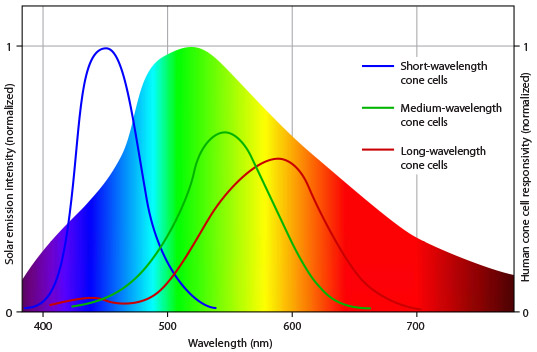
\includegraphics[width=0.8\textwidth]{images/sun_and_vision.jpg}
			\caption{Оптическая система глаза}
		\end{figure}
		\note{
			Заметки
			
		}
	\end{frame}

	\begin{frame}{Функция-согласовывания-цвета-МКО-1931}
		\begin{columns}
			\begin{column}{0.4\textwidth}
				\[	
					X= \int_{380}^{780} I(\lambda)\,\overline{x}(\lambda)\,d\lambda
					\]
					\[
						Y= \int_{380}^{780} I(\lambda)\,\overline{y}(\lambda)\,d\lambda
						\]
						\[
							Z= \int_{380}^{780} I(\lambda)\,\overline{z}(\lambda)\,d\lambda
						\]
			\end{column}
			\begin{column}{0.6\textwidth}
				\begin{figure}
					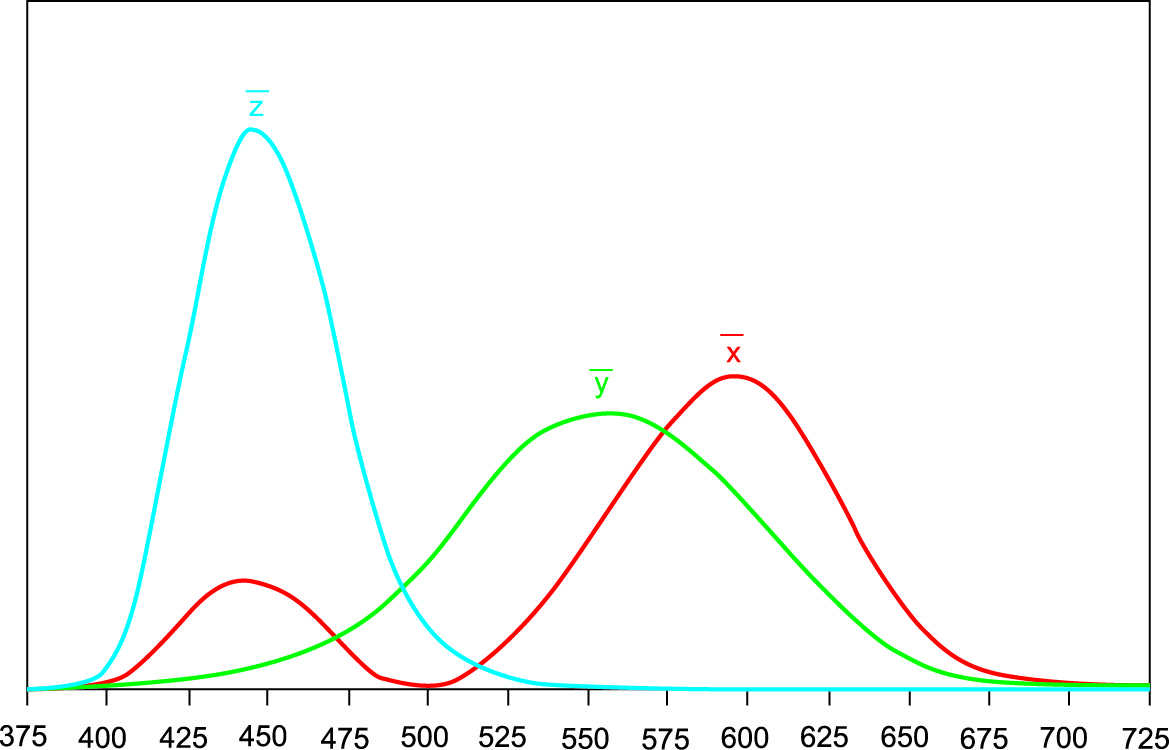
\includegraphics[width=\textwidth]{images/Функция-согласовывания-цвета-МКО-1931.jpg}
					\caption{Функция согласовывания цвета}
				\end{figure}
			\end{column}
		\end{columns}
		\note{
			Международная комиссия по освещению (МКО) — старейшая международная организация по вопросам света и освещения, основанная в 1913 г. МКО является высшим авторитетом по вопросам освещения, признанным Международной организацией по стандартизации (ISO) и Международной электротехнической комиссией (IEC) как международный орган по стандартизации в области освещения. 

			Международная комиссия по освещению (англ. International Commission on Illumination, именуется также CIE по аббревиатуре французского наименования — фр. Commission internationale de l'éclairage, в русскоязычных источниках используется аббревиатура МКО) — международный орган, ведущий разработку технических стандартов в области света, освещения, цвета и цветовых пространств. Создана в 1913 году в качестве преемника Международной комиссии по фотометрии (фр. Commission Internationale de Photométrie).
		}
	\end{frame}

	\begin{frame}{Диаграмма цветности цветового пространства МКО-1931}
		\begin{columns}
			\begin{column}{0.4\textwidth}
				Если формально построить сечение пространства XYZ плоскостью 
				\[X+Y+Z=const,\]
				то можно две оставшиеся линейно-независимыми координаты записать в виде				
				\[x=X/(X+Y+Z)\]
				\[y=Y/(X+Y+Z)\]
			\end{column}
			\begin{column}{0.6\textwidth}
				\begin{figure}
					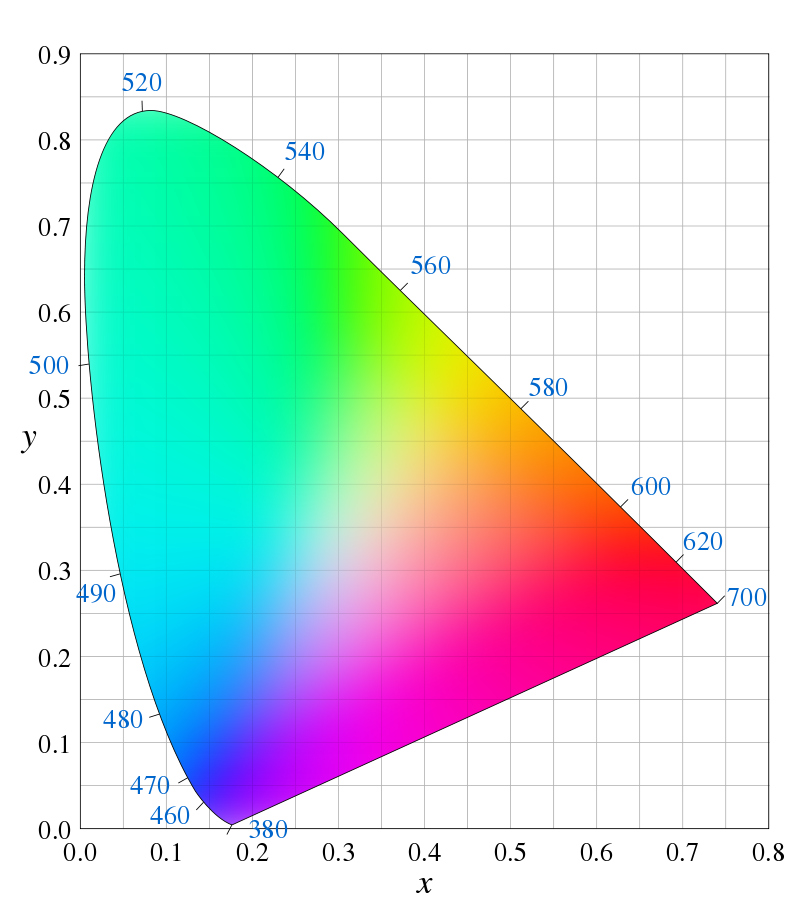
\includegraphics[width=0.7\textwidth]{images/CIExy1931_fixed.png}
					\caption{ Хроматическая диаграмма}
				\end{figure}
			\end{column}
		\end{columns}



		\note{
			Заметки
		}
	\end{frame}

	\begin{frame}{Сравнение различных стандартов цветового спектра в пространстве цветов МКО-1931}
		
		\begin{figure}
			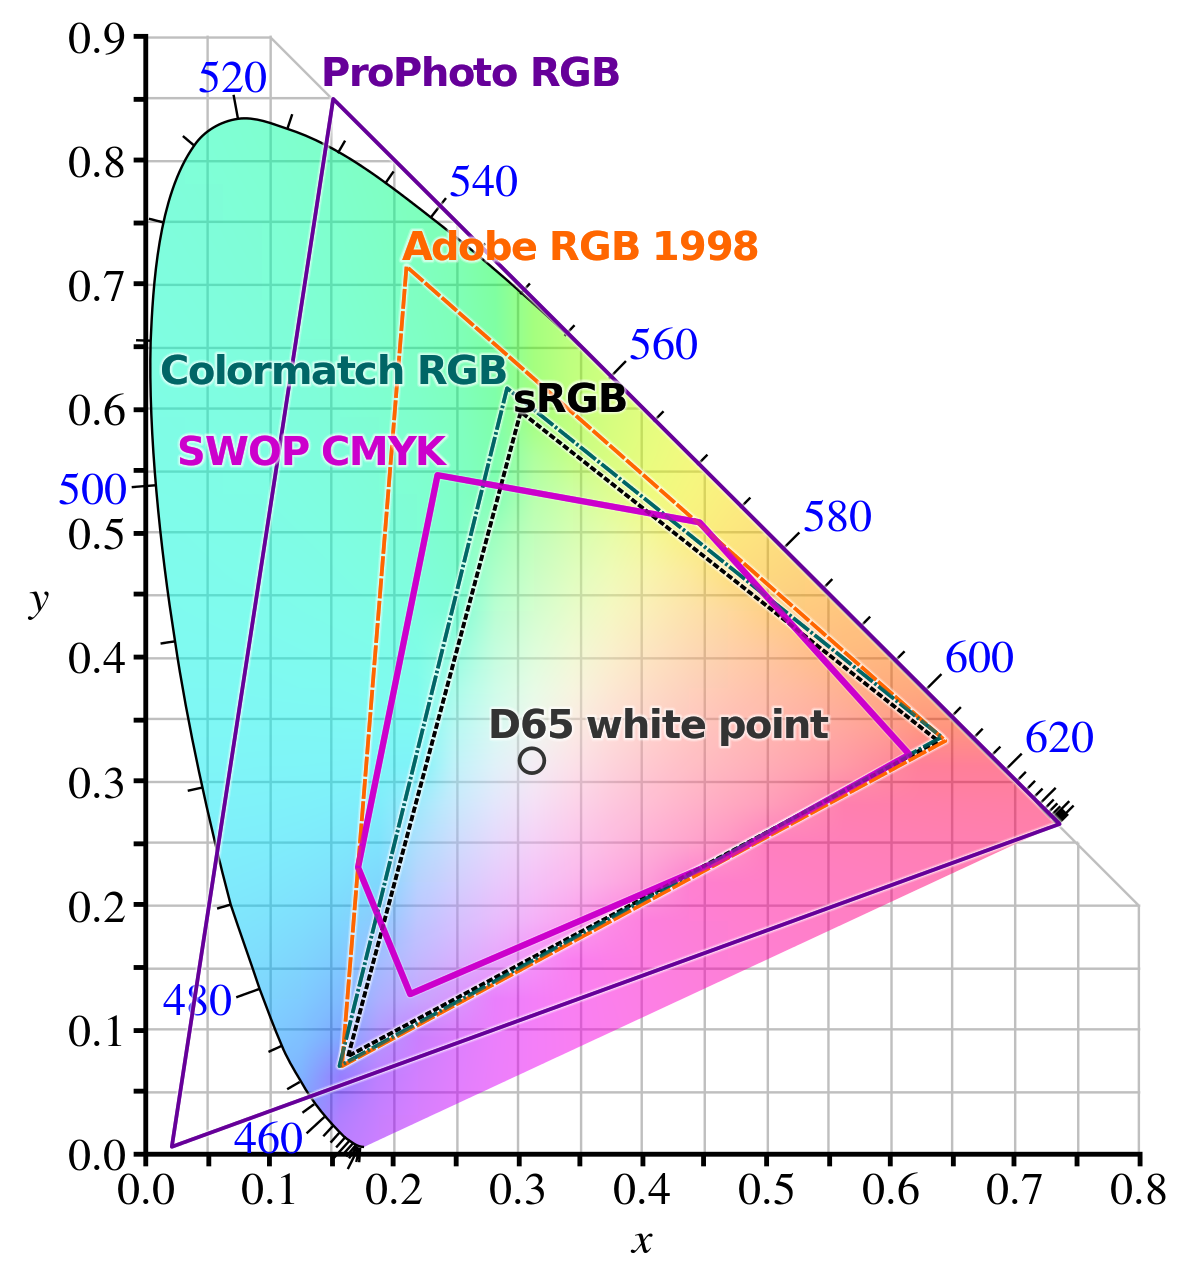
\includegraphics[width=0.45\textwidth]{images/CIE1931xy_gamut_comparison.png}
			\caption{Область цветов sRGB в сравнению с альтернативными стандартами}
		\end{figure}
		\note{
{\tiny

			Пример. Для перевода линейных значений из пространства XYZ (CIE 1931 color space) в sRGB используется следующая матрица:
		\[
			\begin{bmatrix}
				R_\mathrm{linear}\\G_\mathrm{linear}\\B_\mathrm{linear}
			\end{bmatrix}=
				\begin{bmatrix}
					3.2406&-1.5372&-0.4986\\
					-0.9689&1.8758&0.0415\\
					0.0557&-0.2040&1.0570
				\end{bmatrix}
				\begin{bmatrix}
					X \\ 
					Y \\ 
					Z 
					\end{bmatrix}
					\]
					Здесь 
					$R_\mathrm{linear}$ , $G_\mathrm{linear}$ и $B_\mathrm{linear}$
 определены в диапазоне $[0,1]$. 
%  Координаты белой точки, таким образом, составляют (X,Y,Z = 0.9505, 1.0000, 1.0890).

Затем для каждой компоненты цвета используется формула
					\[
						C_\mathrm{srgb}=\begin{cases}
							12.92C_\mathrm{linear}, & C_\mathrm{linear} \le 0.0031308\\
							1.055C_\mathrm{linear}^{1/2.4}-0.055, & C_\mathrm{linear} > 0.0031308
						\end{cases}
						\]

					Эти значения также находятся в диапазоне $[0, 1]$ и для перевода в $[0, 255]$ их нужно умножить на 255 и округлить.

					sRGB (standard RGB, 1996) создан совместно HP и Microsoft в 1996 году для унификации использования модели RGB в мониторах, принтерах и Интернет-сайтах.
					Adobe RGB (1998) --- разработано компанией Adobe Systems, Inc. охватывает около 50\% видимых цветов.
					ProPhoto RGB (2013)  --- Кодак, более 90\% охвата видимых цветов, недостатков этого цветового пространства является то, что около 13\% представленных цветов — это мнимые цвета, которые не существуют, и невидимые цвета.
					
					SWOP is a color reproduction Specification for web offset lithography.
}
		}
	\end{frame}

	\begin{frame}{ЦВЕТОВАЯ ТЕМПЕРАТУРА. }
		\begin{figure}
			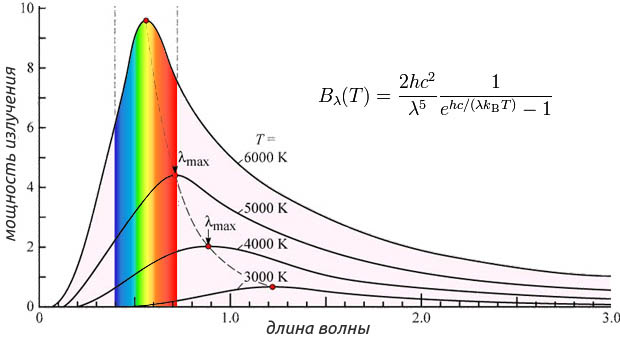
\includegraphics[width=0.9\textwidth]{images/Спектральное-распределение-излучения-абсолютно-черного-тела.jpg}
			\caption{
				Спектральные распределения интенсивности излучения абсолютно чёрного тела по длинам волн, измеренные при разных температурах
				}
		\end{figure}
		\note{
			Белый свет имеет особые цветовые характеристики. Существует
много оптических спектров излучения, при помощи которых можно создать
излучение белого цвета. Среди этих спектров можно выделить спектр
излучения абсолютно чёрного тела, часто называемого излучением Планка.

Данный спектр лежит в основе однозначного и очень полезного стандарта,
позволяющего описывать спектр излучения при помощи одного
единственного параметра --- цветовой температуры.

В качестве независимого стандарта, характеризующего белый свет,
часто используют спектр излучения абсолютно чёрного тела, определяемый
только одним параметром --- температурой излучающего тела. Первым
формулу, описывающую спектральную плотность светимости чёрного тела
с заданной температурой, вывел Макс Планк в 1900 г.

Закон смещения Вина
\[
	\lambda_\text{max} = 2898/T,
	\]	
		}
	\end{frame}

	\begin{frame}{Кривая излучения (кривая Планка) абсолютно черного тела в цветовом пространстве МКО 1931}
	\begin{figure}
		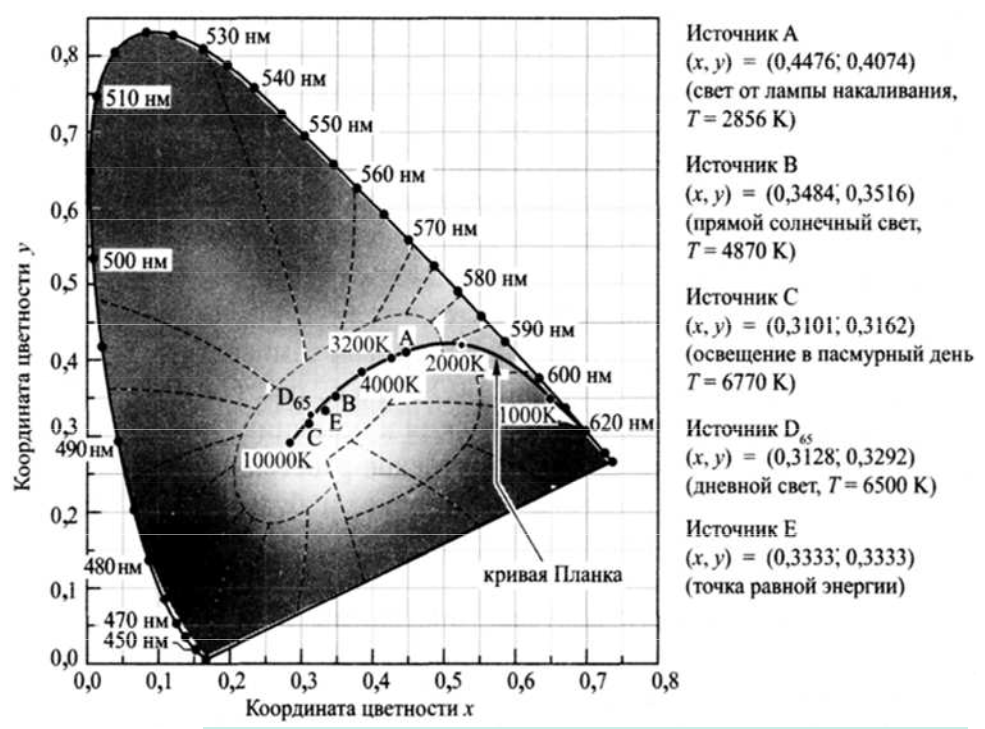
\includegraphics[width=0.6\textwidth]{images/Цветовая-диаграмма-и-кривая-Планка.png}
		\caption{
			Цветовая диаграмма, на которой показаны кривая Планка и
положение стандартных источников излучения белого света $A$ , $B$ , $C$ и $D_{65}$
			}
	\end{figure}
	\note{
		С ростом температуры чёрного тела положение его излучения на диаграмме
		сдвигается из области красных волн ближе к центру диаграммы.

		С ростом температуры цвет свечения чёрного тела меняется от красного до голубовато-белого (красный – оранжевый – жёлтовато-белый – белый – голубовато-белый)
	
		Если источник белого света не попадает на кривую Планка, для его
описания используется коррелированная цветовая температура.
		}
\end{frame}
	
	\begin{frame}{Tone Mapping и HDR}
		\begin{figure}
			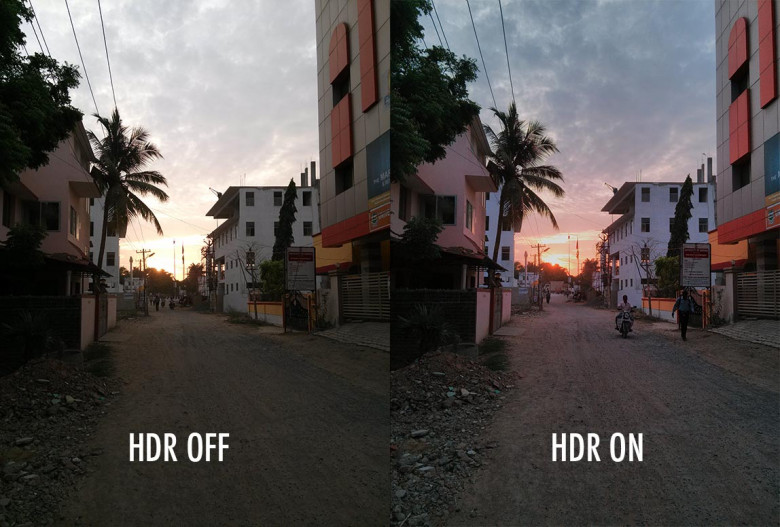
\includegraphics[width=0.7\textwidth]{images/HDR-ON-OFF.jpeg}
			\caption{
				SDR (Standard Dynamic Range) и HDR (High Dynamic Range) в сравнении
				}
		\end{figure}
		\note{
			HDR - это сокращение обозначения "High Dynamic Range" - расширенный динамический диапазон. Эта технология улучшает детализацию изображения в самых темных и светлых сценах. Она делает картинку на экране более естественной и реалистичной даже в широком диапазоне контрастности.

			Динамическое отображение тонов (Dynamic Tone Mapping) — это вычислительный процесс, в котором используется алгоритм для сегментации и анализа исходного изображения HDR в режиме реального времени и переназначения или изменения уровней теней, средних тонов и светлых участков в определенных областях изображения автоматически на основе коэффициентов контрастности сцены. Целью этого процесса является максимально простое создание красивого и готового изображения без участия человека. Это автоматизированное редактирование изображений для потребительской фотографии и видеосъемки в массовом масштабе.
		}
	\end{frame}

	\begin{frame}{Tone Mapping и HDR}
		\begin{figure}
			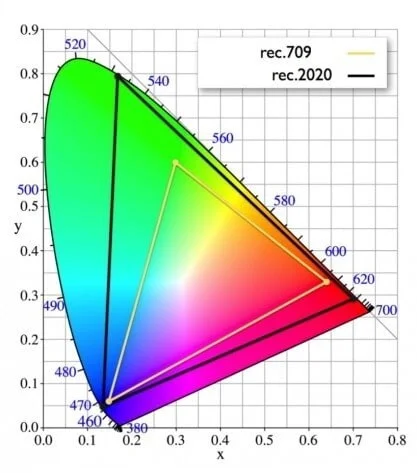
\includegraphics[width=0.45\textwidth]{images/rec.709-vs-rec.2020.png}
			\caption{
				Сравнение rec.709 rec.2020
				}
		\end{figure}
		\note{
			Почему фотки с последних моделей телефона отображают цвета на экране по-другому?

			SDR формат базируется на колориметрических параметрах, описанных в Rec. ITU-R BT. 709. (совпадает sRGB, 35.9\%) Они охватывают всего лишь 35.9\% видимого человеческим глазом спектра системы CEI 1931. 
			
			В свою очередь HDR использует цветовые параметры Rec.ITU-R BT. 2020 (близко к Adobe Wide Gamut RGB, у которого охват спектра примерно 77.6\%), охватывающие 75.8\% спектра.
		}
	\end{frame}

	\begin{frame}{Глубина цвета}
		\begin{figure}
			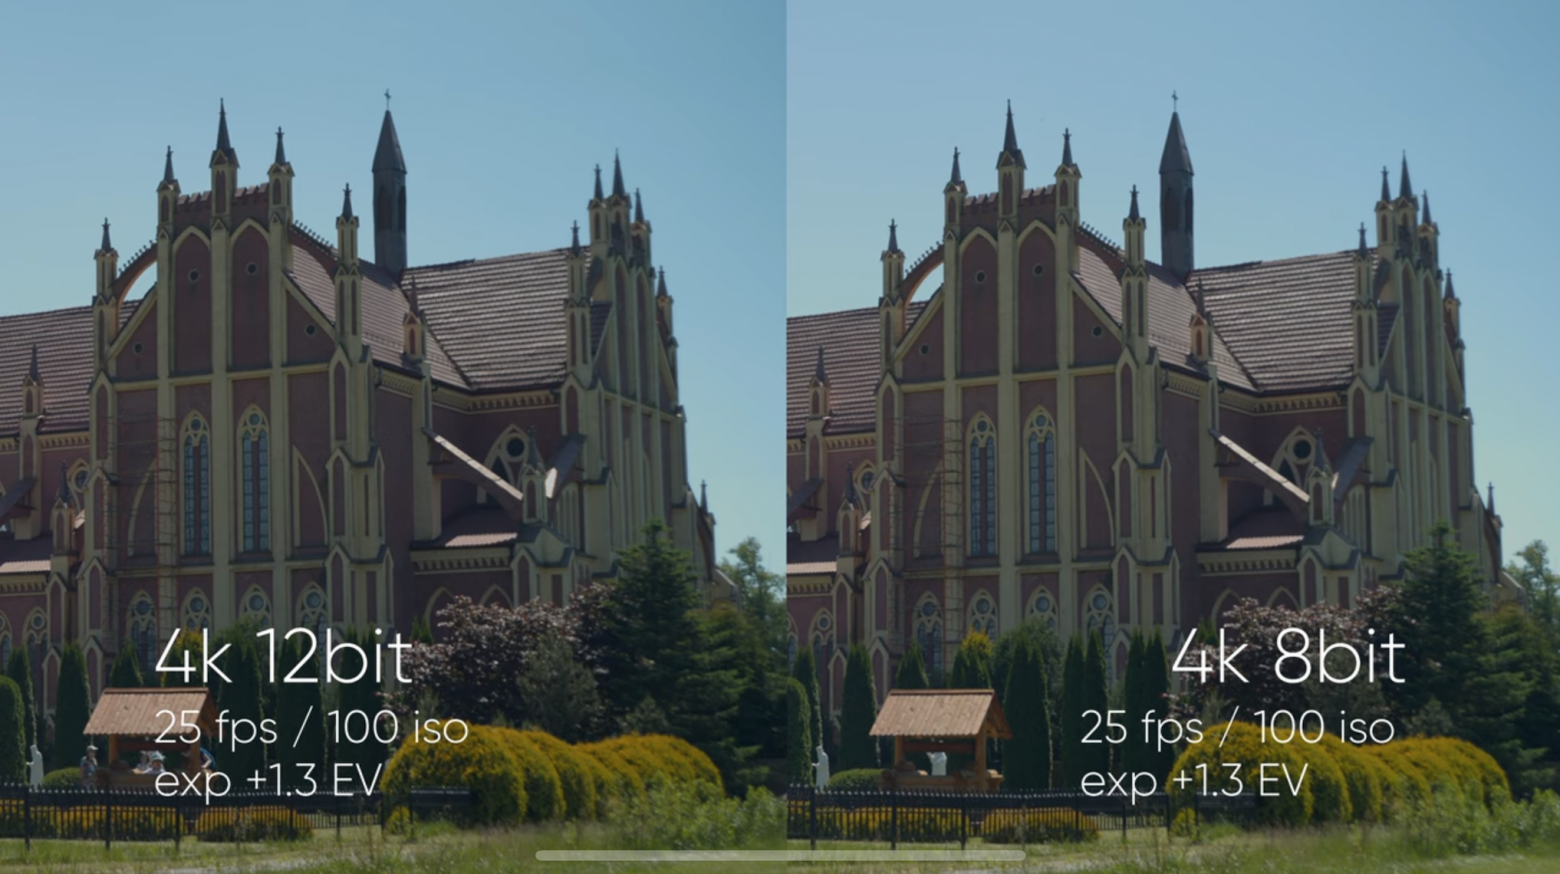
\includegraphics[width=0.9\textwidth]{images/HDR_COMPARISON.png}
			\caption{
				Пример фотоснимков, имеющих разную глубину цвета
				}
		\end{figure}
		\note{
			\begin{figure}
				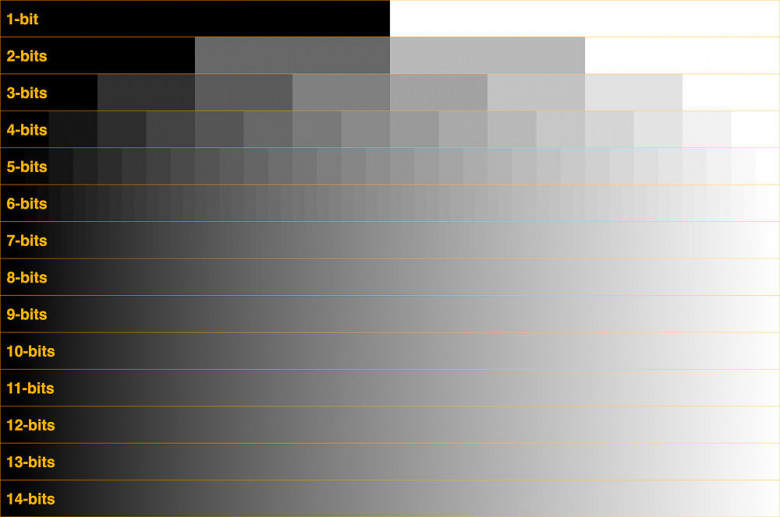
\includegraphics[width=0.7\textwidth]{images/HDR-плавность-градиента.jpg}
				\caption{
					Влияние "битность" цвета на плавность градиента
					}
			\end{figure}
		}

	\end{frame}

	\if 0
	\begin{frame}{Методы представления графической информации}
		
		\centering
		\textbf{Основные направления}
		
		\begin{columns}
			\begin{column}{0.3\textwidth}
				
				Растровая графика
				
				Блоки универсальных элементов
				
				pixel (pix element)
				экранный (ppi – pixels per inch)
				печатный (dpi – dots per inch)
				
				% \begin{figure}
				% 	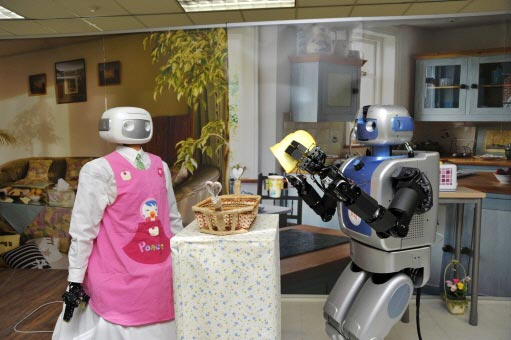
\includegraphics[width=\textwidth]{images/Computer_vision.png}
				% 	\caption{Семейная пара}
				% \end{figure}
			\end{column}
			
			\begin{column}{0.4\textwidth}
				
				Векторная графика

				Регулярные структуры
				point, line, triangle etc.

				% \begin{figure}
				% 	
\includegraphics[width=\textwidth]{images/Utah_teapot.png}
				% 	\caption{Чайник Юта}
				% \end{figure}
				
			\end{column}
			
			\begin{column}{0.3\textwidth}
				
				Фрактальная графика

				Фигуры
				
				% \begin{figure}
				% 	\includegraphics[width=\textwidth]
				% 	{images/Lenna_test_image.png}
				% 	\caption{Лена Сёдерберг}
				% \end{figure}
				
			\end{column}
		\end{columns}

	\end{frame}
	\fi
\end{document}